\subsection{Aufgabe 2}
\subsubsection{Die Abhängigkeit zwischen Photostrom und Intensität des Lichts}
Als erstes wollen wir in diesem Versuch den Zusammenhang zwischen der Intensität des Photostroms und der Anzahl der aus dem Metall herausgelösten Elektronen untersuchen. Dazu justieren wir die Photozelle so, dass nur die indigoblaue Spektrallinie (\(\lambda\) = 435,8 nm) durch den Spalt der Photozelle gelangt und schließen den variablen Spalt. Zur Messung öffnen wir den variablen Spalt in 1/100 mm Schritten und notieren uns den Photostrom. Die Saugspannung \(U_{saug}\) blieb im Verlaufe der Messung konstant bei +8V.\\
In der folgenden Tabelle sind unsere Messwerte aufgelistet, welche wir in Abbildung 1 grafisch dargestellt haben.\\

\begin{center}
\(d [mm]\) & \(I [\my A]\) \\ 
\(2.46\) & \(0.25\) \\ 
\(2.45\) & \(0.3\) \\ 
\(2.44\) & \(0.3\) \\ 
\(2.43\) & \(0.3\) \\ 
\(2.42\) & \(0.3\) \\ 
\(2.41\) & \(0.3\) \\ 
\(2.4\) & \(0.4\) \\ 
\(2.39\) & \(0.5\) \\ 
\(2.38\) & \(5.68\) \\ 
\(2.37\) & \(10.6\) \\ 
\(2.36\) & \(16.06\) \\ 
\(2.35\) & \(31.4\) \\ 
\(2.34\) & \(39.8\) \\ 
\(2.33\) & \(47\) \\ 
\(2.32\) & \(53.9\) \\ 
\(2.31\) & \(61.7\) \\ 
\(2.3\) & \(73.48\) \\ 
\(2.29\) & \(79.6\) \\ 
\(2.28\) & \(87.3\) \\ 
\(2.27\) & \(96.7\) \\ 
\(2.26\) & \(106\) \\ 
\(2.25\) & \(117\) \\ 
\(2.24\) & \(127\) \\ 
\(2.23\) & \(143\) \\ 
\(2.22\) & \(151\) \\ 
\(2.21\) & \(161\) \\ 
\(2.2\) & \(180\) \\ 
\(2.19\) & \(208\) \\ 
\(2.18\) & \(224\) \\ 
\(2.17\) & \(224\) \\ 
\(2.16\) & \(240\) \\ 
\(2.15\) & \(259\) \\ 
\(2.14\) & \(291\) \\ 
\(2.13\) & \(287\) \\ 
\(2.12\) & \(309\) \\ 
\(2.11\) & \(328\) \\ 
\(2.1\) & \(345\) \\ 
\(2.09\) & \(358\) \\ 
\(2.08\) & \(370\) \\ 
\(2.07\) & \(382\) \\ 
\(2.06\) & \(393\) \\ 
\(2.05\) & \(414\) \\ 
\(2.04\) & \(427\) \\ 
\(2.03\) & \(440\) \\ 
\(2.02\) & \(444\) \\ 
\(2.01\) & \(444\) \\ 
\(

\captionof{table}{Rohmesswerte der Spaltbreite d und des Photostroms}
\end{center}

\begin{center}
\begin{minipage}{\linewidth}
\centering
\makebox[0cm]{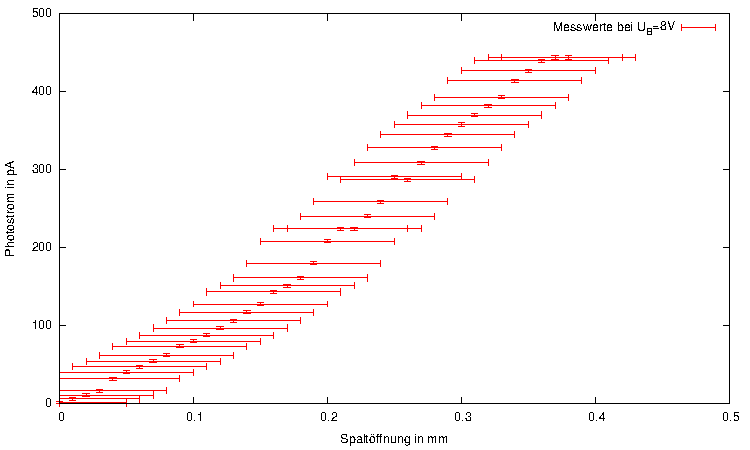
\includegraphics[width=\textwidth]{graphen/2a}}
\label{ips}
\end{minipage}
\end{center}

Wie deutlich erkennbar ist, herrscht ein linearer Zusammenhang zwischen der Intensität des einfallenden Lichts und dem Photonenstrom. Der Fehlerwert der Spaltöffnung muss anhand der Ablesegenauigkeit geschätzt werden.

\subsubsection{Die Abhängigkeit zwischen der Bremsspannung und\\ der Intensität}

